\chapter{Introduction}\label{ch:intro}

Every new generation of cellular network technologies comes with a new set of
requirements, dictated by the trends in the use of the mobile connectivity. A
common requirement to every single generation is their striving for higher data
rates and greater power efficiency. This motivates research and techology
innovation in order to achieve the goals set for each generation.


The research associated usually requires revisiting old paradigms used in
previous generations, and updating them with novel ideas.


The \emph{release 7} of the \gls{3gpp} \gls{3g} specifications \cite{3gpprel7},
also known as \gls{hspa+}, included the use of \gls{mimo} as a means to increase
the transmission rates.


\emph{Release 8}, more well known by its commercial name \gls{lte}
\cite{3gpplte}, introduced a new physical layer, based on \gls{ofdm} instead of
\gls{wcdma} as in \gls{3g}. Although the rates attainable with \gls{wcdma} may
be comparable to those obtained with \gls{ofdm}, the latter provides a much
easier equalization mechanism that makes dealing with multipath channels a
simpler task. Apart from that \gls{ofdm} provides a higher flexibility in the
resource allocation and user and enables the use of \gls{ofdma}.

\gls{lte} did not meet the requirements issued by the \gls{itur} \gls{imta}
radio interface \cite{imta} for what is known as \gls{4g} though.

The introduction of \gls{ltea} in \emph{release 10} of the LTE specification
\cite{3gppltea} met the requirements to be considered an \gls{imta} system. The
main novelties included in \gls{ltea} are \gls{ca}, enhanced use of MIMO
techniques and support for \glspl{rn}.

\emph{Release 11} \cite{3gpprel11} included in the specification the support for
\gls{comp} operation. \gls{comp} was included in order to improve the network
performance at cell edges, for it uses several transmitters to provide
coordinated transmission in the downlink, and a number of receivers to provide
coordinated reception in the uplink.

With \gls{ltea} standardized and its deployment already ongoing, further
releases of \gls{ltea} still continue but standards bodies and industry are
already looking ahead at the future \gls{5g}, and so is doing the research
world. Even though there is no definite idea about what \gls{5g} will be, it is 
clear what it will \emph{not} be, an incremental advance on \gls{4g}. It needs
to be a paradigm shift \cite{andrews14}.

The new \gls{5g} systems will be characterized by being heterogeneous, what is
known as \glspl{hetnet}, formed by multiple small cells, using different radio
access technologies \cite{chin14}. One of the main problems for \glspl{hetnet}
is inter-cell interference, because of the possible presence of unplanned
deployment of small cells, and the irregular shape of the cells. Hence the importance of interference coordination techniques.

\begin{figure}[t]
    \centering
    \begin{subfigure}[b]{0.45\textwidth}
            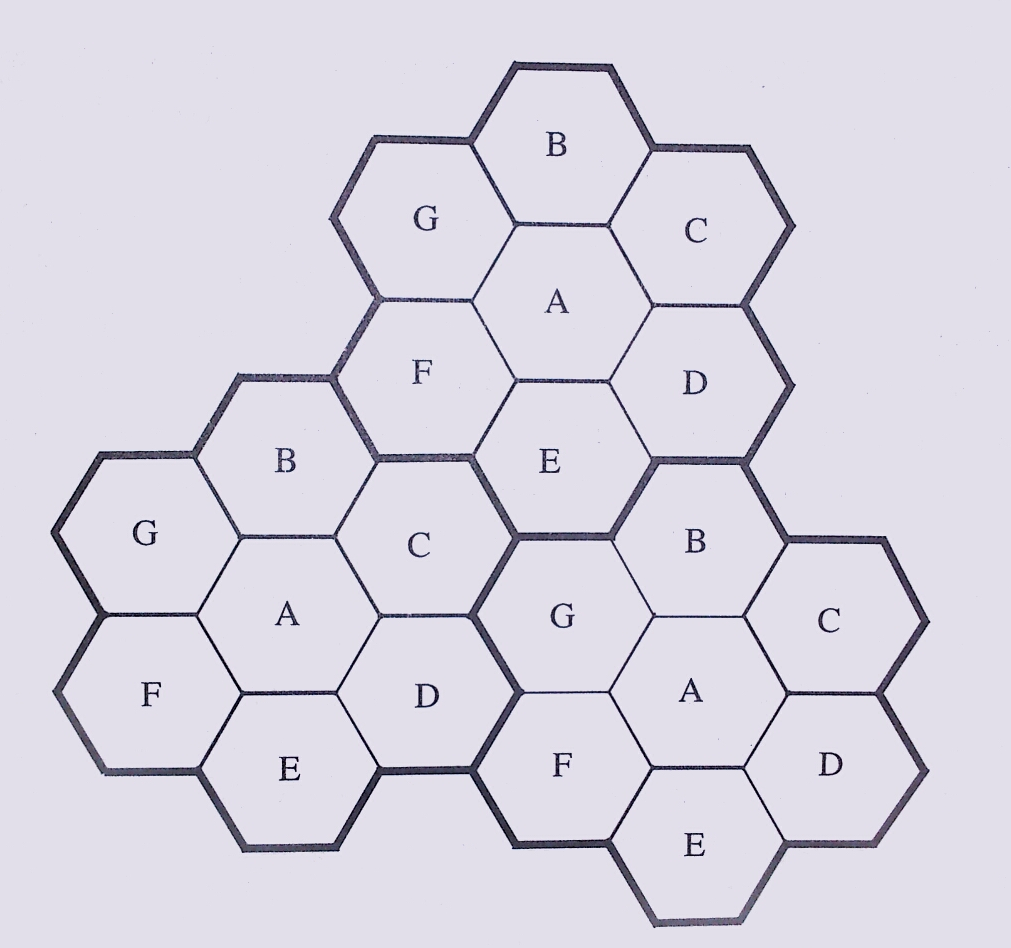
\includegraphics[width=\textwidth]{./01.introduction/img/frequency_reuse.png}
        \caption{Frequency reuse factor of $1 / 7$.}
        \label{fig:freuse}
    \end{subfigure}
    % Comment out the line break that is introduced with the blank line
    % so that it does not put the images one on top of the other...
    \begin{subfigure}[b]{0.45\textwidth}
        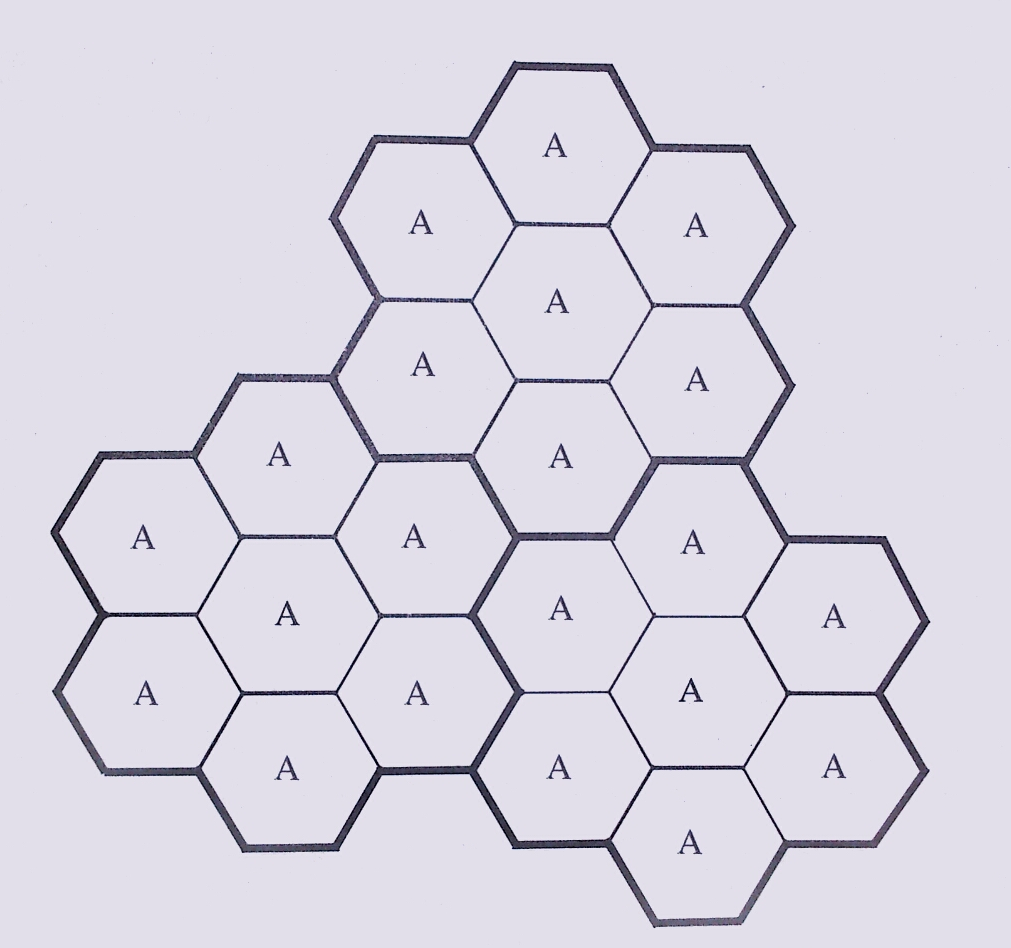
\includegraphics[width=\textwidth]{./01.introduction/img/universal_freq_reuse.png}
        \caption{Frequency reuse factor of $1$. {\color{red} DO NOT FORGET TO NOT EMPHASIZE THE 7-CELL CLUSTERS BUT EACH CELL INDIVIDUALLY}}
        \label{fig:ufreuse}
    \end{subfigure}
    \caption{Different frequency planning options}
    \label{fig:freq_plan}
\end{figure}

Current \gls{mimo} systems used in cellular networks are not achieving the
expected performance predicted by the initial theoretical works. The main reason
for this is the interference that is present naturally in cellular systems when
all cells share the same spectrum for the tranmissions. The effect of this
interference is a reduction of the \gls{sinr} experienced by the users, highly
reducing the advantages that \gls{mimo} could potentially deliver.

The conventional approach for cellular networks was to perform a careful
frequency planning in order to avoid the interference among neighboring cells.
Clusters of $N$ cells were grouped together, and assigned $N$ frequency bands to
be used, and the pattern is repeated for different clusters, yielding what is
called a \emph{frequency reuse factor} of $1/N$, as exemplified in
\reff{fig:freuse}.

The problem that this poses is that the available spectrum must be split, which
is an inherent inefficiency in the use of the resources.

A different option consists on a system where all the cells share a common
spectrum, so that all of them can use the full amount of resources available.
This is called \gls{ufr}, and a graphical description can be seen in
\reff{fig:ufreuse}.

It is in this kind of networks that the need for coordination among cells
arises, as every cell will interfere with the rest of the cells in the system
reducing the \gls{sinr} operating point of the users.

In the search for higher data rates and a more efficient use of the resources,
\gls{ufr} is a must to make the most out of the scarce resource that the radio
frequency spectrum is. Therefore, ``A new look at the interference''
\cite{gesbert10} is needed. The conventional concept of the interference as
being an impairment needs to shift to a new point of view where the interference
can be used to improve the overall performance of the network. A joint
optimization of the resources among all the cells is required in order to
globally improve the perfomance of the system \cite{gesbert07}.

The \gls{comp} operation considered in \cite{3gpprel11} is just a part of a much
broader field of multicell cooperation or coordinated communications where
several cells are assumed to cooperate, in the sense that they take measures in
order to alleviate to a certain degree the level of interference introduced into
other parts of the network, or the use of that interference to their advantage.

Intuitively, the best strategy should be to allow all the \glspl{bs} in the
network to cooperate, what is known as \emph{global coordination}. Even though
it may seem that global coordination may solve all the problems of frequency
planning and resource allocation, it cannot be ignored that it comes at a
non-negligible cost. The \glspl{bs} in the network may need to interchange
information in order to cooperatively transmit the information to all the users
in the system. The amount of information that needs to be exchanged grows out of
control with the size of the network, \ie the number of \glspl{bs} that form the
system. The result of this is that the capacity required to transmit this
information renders the alleged solution useless. Not only are the backhaul
transmission capabilities required prohibitive, but also tight synchronization
among the \glspl{bs} becomes a challenge, and channel information gathering
becomes a cumbersome task. Apart from this, theoretical works \cite{lozano13}
have unveiled intrinsic limitations of cooperation, whose benefits do not
unboundedly grow with the size of the coordination group.

For all these reasons, clustering appears as a means to cope with the
limitations of global coordination. In clustering, the coordination is not
performed among all the \glspl{bs} in the network but, instead, small groups, or
clusters, are formed and the cooperation takes place locally within the cluster.
This greatly reduces the amount of control information that should be handled by
the backhaul. Also, the reduced size of the group makes the system work at an
operating point where the natural limitations mentioned in \cite{lozano13} do
not affect the performance of the network.

\begin{figure}[t]
    \centering
    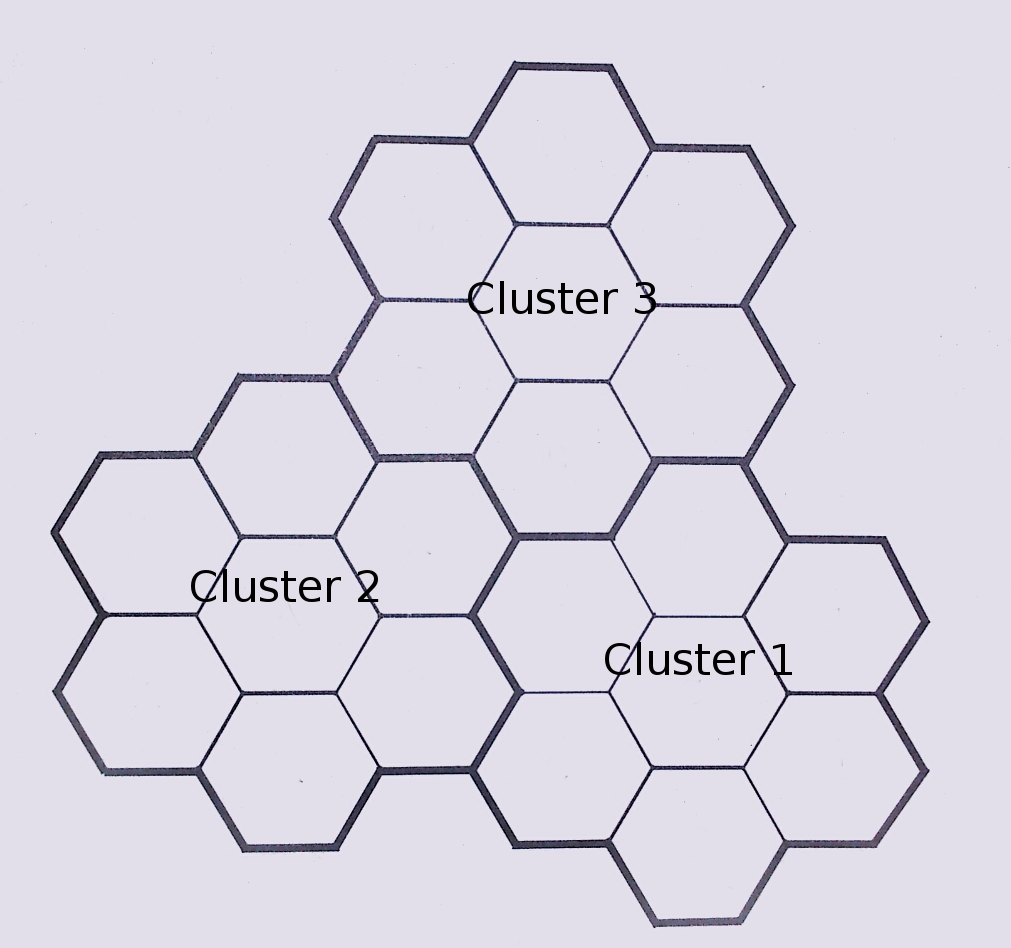
\includegraphics[width=0.45\textwidth]{./01.introduction/img/clustered_network.png}
    \caption{Clustered network scenario.}
    \label{fig:clustered_network}
\end{figure}

A schematic representation of a clustered network can be seen in
\reff{fig:clustered_network} where three clusters of seven cells are shown.

Grouping the cells in reduced size clusters has an important drawback: If the
cooperation is done within a cluster and neighboring clusters are not
coordinated in any way, there would be, again, unhandled interference, albeit
not the same as in the uncoordinated scenario.

This thesis focuses on a clustered cellular network where \gls{bd} is used for
coordination within each cluster. The performance of the network, in terms of
achievable rate and fairness considerations, is analyzed and its dependence on
several parameters of the network is studied. Also, mechanisms to deal with the
interference, resulting from clustering, are presented.

The organization of the document is as follows:

\begin{itemize}
    \item In \verb+\refc{ch:state_art}+ a compilation of different alternatives for
        coordination, as well as for clustering, found in the literature are
        presented and described.
    \item \verb+\refc{ch:system_model}+ presents the system model used throughout the
        dissertation, and describes in detail \gls{bd} and the power allocation
        strategies used in the rest of the work.
    \item \verb+\refc{ch:achiev_rates}+ analyzes the performance of a cellular network,
        in terms of the mean achievable rate as a function of the cluster size,
        when using \gls{bd} for coordination within each cluster, and taking
        into account the interference due to external clusters. An analytical
        expression for the mean achievable rate is developed and the optimum
        cluster size is obtained.
    \item \verb+\refc{ch:rate_statistics}+ considers the fairness of the system, and
        studies the variability of the rate, as a complement to the mean
        obtained in \verb+\refc{ch:achiev_rates}+. The behavior of the rates is shown
        to follow almost exactly a Gamma distribution.
    \item The pernicious effect of the \gls{oci} in the rates is introduced in
        \verb+\refc{ch:adaptive_schedule}+, and a mechanism to deal with it, based on
        a mixed tranmission strategy and on a scheduling algorithm, is
        presented.
    \item Finally, some conclusions are presented in \verb+\refc{ch:conclusions}+, and
        future research topis are discussed.
\end{itemize}
